\documentclass[12pt, a4paper]{article}

% utilizzato per inserire foto
\usepackage[]{graphicx}

% Utilizzato per convertire alcuni testi di default in italiano
\usepackage[italian]{babel}
% permette agli hypertext di essere cliccabili
\usepackage{hyperref}
\hypersetup{
    colorlinks,
    citecolor=black,
    filecolor=black,
    linkcolor=black,
    urlcolor=magenta
}

% FONT
\usepackage{newtxtext}
\usepackage[margin=3cm]{geometry}

% interlinea
\usepackage{setspace}
\renewcommand{\baselinestretch}{1.5} 

\newcommand{\meskip}{\medskip \\}
\newcommand{\bskip}{\bigskip \\}

\usepackage{enumitem}

% ############ JUSTIFY ############
\tolerance=1
\emergencystretch=\maxdimen
\hyphenpenalty=10000
\hbadness=10000
% #################################

\title{
    
\includegraphics[width=.8\textwidth]{images/LOGO.png}\\
    \textbf{Business Plan}
}
\date{}
\author{}

\begin{document}

\maketitle

\newpage

\tableofcontents

\newpage

\section{Descrizione dell'impresa}
La nostra startup è stata fondata con un obiettivo chiaro: offrire un'esperienza enologica eccezionale a tutti gli appassionati del vino.
Siamo fermamente convinti che il vino non sia solo una bevanda, ma un'arte che merita di essere scoperta e apprezzata appieno.\meskip
Attraverso la nostra piattaforma online, abbiamo creato un ambiente virtuale in cui i nostri clienti possono immergersi nel meraviglioso mondo del vino. Offriamo loro l'opportunità di esplorare un vasto assortimento di vini provenienti da diverse regioni e cantine, consentendo loro di ampliare le loro conoscenze e scoprire nuovi gusti. Inoltre, forniamo recensioni autentiche e affidabili, garantendo ai nostri clienti una guida preziosa nella scelta del vino più adatto alle loro preferenze.\meskip
Sappiamo che la comodità è un elemento fondamentale nella vita di oggi, quindi ci assicuriamo che i nostri clienti possano godere di un'esperienza di acquisto senza problemi. Grazie al nostro sistema di ordini online, possono selezionare i loro vini preferiti e riceverli comodamente a casa propria. E per garantire che ogni bottiglia arrivi in condizioni ottimali, abbiamo stretto partnership con servizi di spedizione veloci e affidabili.\meskip
Ma c'è qualcosa che ci rende davvero speciali.
In Vinovo, mettiamo un'enfasi particolare sulla sostenibilità nel settore vinicolo.
Siamo consapevoli dell'importanza di preservare l'ambiente e lavoriamo solo con produttori che adottano pratiche ecologiche nella produzione dei loro vini.
Ci impegniamo a ridurre l'impatto ambientale, promuovendo l'uso responsabile delle risorse e incoraggiando l'agricoltura sostenibile.\meskip
In sintesi, Vinovo rappresenta molto più di una semplice piattaforma di vendita di vini. Rappresenta un'esperienza enologica completa, in cui la qualità e la sostenibilità si uniscono per offrire ai nostri clienti un viaggio indimenticabile nel mondo del vino. Vogliamo essere il punto di riferimento per tutti coloro che desiderano esplorare l'arte e il piacere di un buon bicchiere di vino, garantendo loro un accesso facile a una selezione vasta e curata.
Unisciti a noi in questo viaggio e lasciati conquistare dalla passione e dall'eccellenza che si cela dietro ogni nostra bottiglia di vino.

\subsection{Vision e mission}
\subsubsection*{Vision}
La nostra visione è quella di trasformare l'esperienza enologica in un viaggio affascinante e coinvolgente, in cui la qualità, la sostenibilità e la scoperta si fondono armoniosamente.
Vogliamo che ogni appassionato del vino possa esplorare e apprezzare i tesori enogastronomici del mondo, guidato dalla curiosità e dalla consapevolezza di fare scelte che rispettino l'ambiente.

\subsubsection*{Mission}
La nostra missione è quella di creare un legame forte tra i produttori di vini di alta qualità e i consumatori desiderosi di vivere un'esperienza enologica autentica.\\
Ci concentriamo sulla qualità dei prodotti, sulla sostenibilità delle pratiche produttive e sulla garanzia di un servizio di spedizione veloce e sicuro.\meskip
Ci adoperiamo attivamente per promuovere la sostenibilità nel settore vinicolo; vogliamo educare i consumatori sull'importanza di fare scelte sostenibili e offrire loro una selezione di vini che rispecchi questi valori.\meskip
Siamo determinati a diventare un punto di riferimento per tutti coloro che cercano\\ un'esperienza enologica autentica, basata sulla scoperta, sulla qualità e sulla sostenibilità.
Vogliamo creare una comunità in cui gli appassionati del vino possano condividere le loro esperienze, imparare dagli esperti del settore e lasciarsi ispirare da nuove tendenze e scoperte enogastronomiche.\meskip
In sintesi, la nostra visione è quella di offrire un'esperienza enologica di qualità, in cui la passione per il vino si unisce alla consapevolezza ambientale.

\subsection{Collaborazioni}
I nostri collaboratori sono una parte fondamentale del successo di Vinovo.
Collaboriamo con una rete diversificata di partner, tra cui ristoranti e locali, produttori di vini e aziende di logistica, che contribuiscono a rendere possibile la nostra missione.\meskip
I ristoranti e i locali con cui collaboriamo sono selezionati con cura per offrire ai nostri clienti un'esperienza culinaria raffinata e in sintonia con i vini di alta qualità presenti sulla nostra piattaforma.
Riconosciamo l'importanza di abbinare il vino ad una cucina di qualità, e la collaborazione con questi partner ci consente di offrire ai nostri clienti un'esperienza completa, in cui i sapori si armonizzano perfettamente.\meskip
Collaboriamo con cantine che mettono passione e impegno nella produzione di vini di alta qualità, rispettando l'ambiente.
Questa collaborazione ci consente di offrire ai nostri clienti una selezione accurata di vini unici e di raccontare le storie dietro ogni etichetta.\meskip
Le aziende di logistica con cui ci associamo sono responsabili della spedizione dei nostri vini.
Siamo consapevoli dell'importanza di garantire che ogni bottiglia arrivi in condizioni ottimali e nel minor tempo possibile.
Le aziende di logistica con cui collaboriamo condividono i nostri alti standard di affidabilità e sicurezza, garantendo che i nostri clienti possano godere dei loro vini preferiti senza preoccupazioni.\meskip
Riconosciamo il valore delle relazioni di collaborazione e crediamo nell'importanza di costruire partnership solide e durature.\meskip
Continueremo a coltivare queste partnership e a cercare nuove opportunità di collaborazione, perché crediamo che insieme possiamo offrire ai nostri clienti un viaggio indimenticabile nel mondo del vino.\newpage

\subsection{Bozza del sito web}
\begin{center}
    \frame{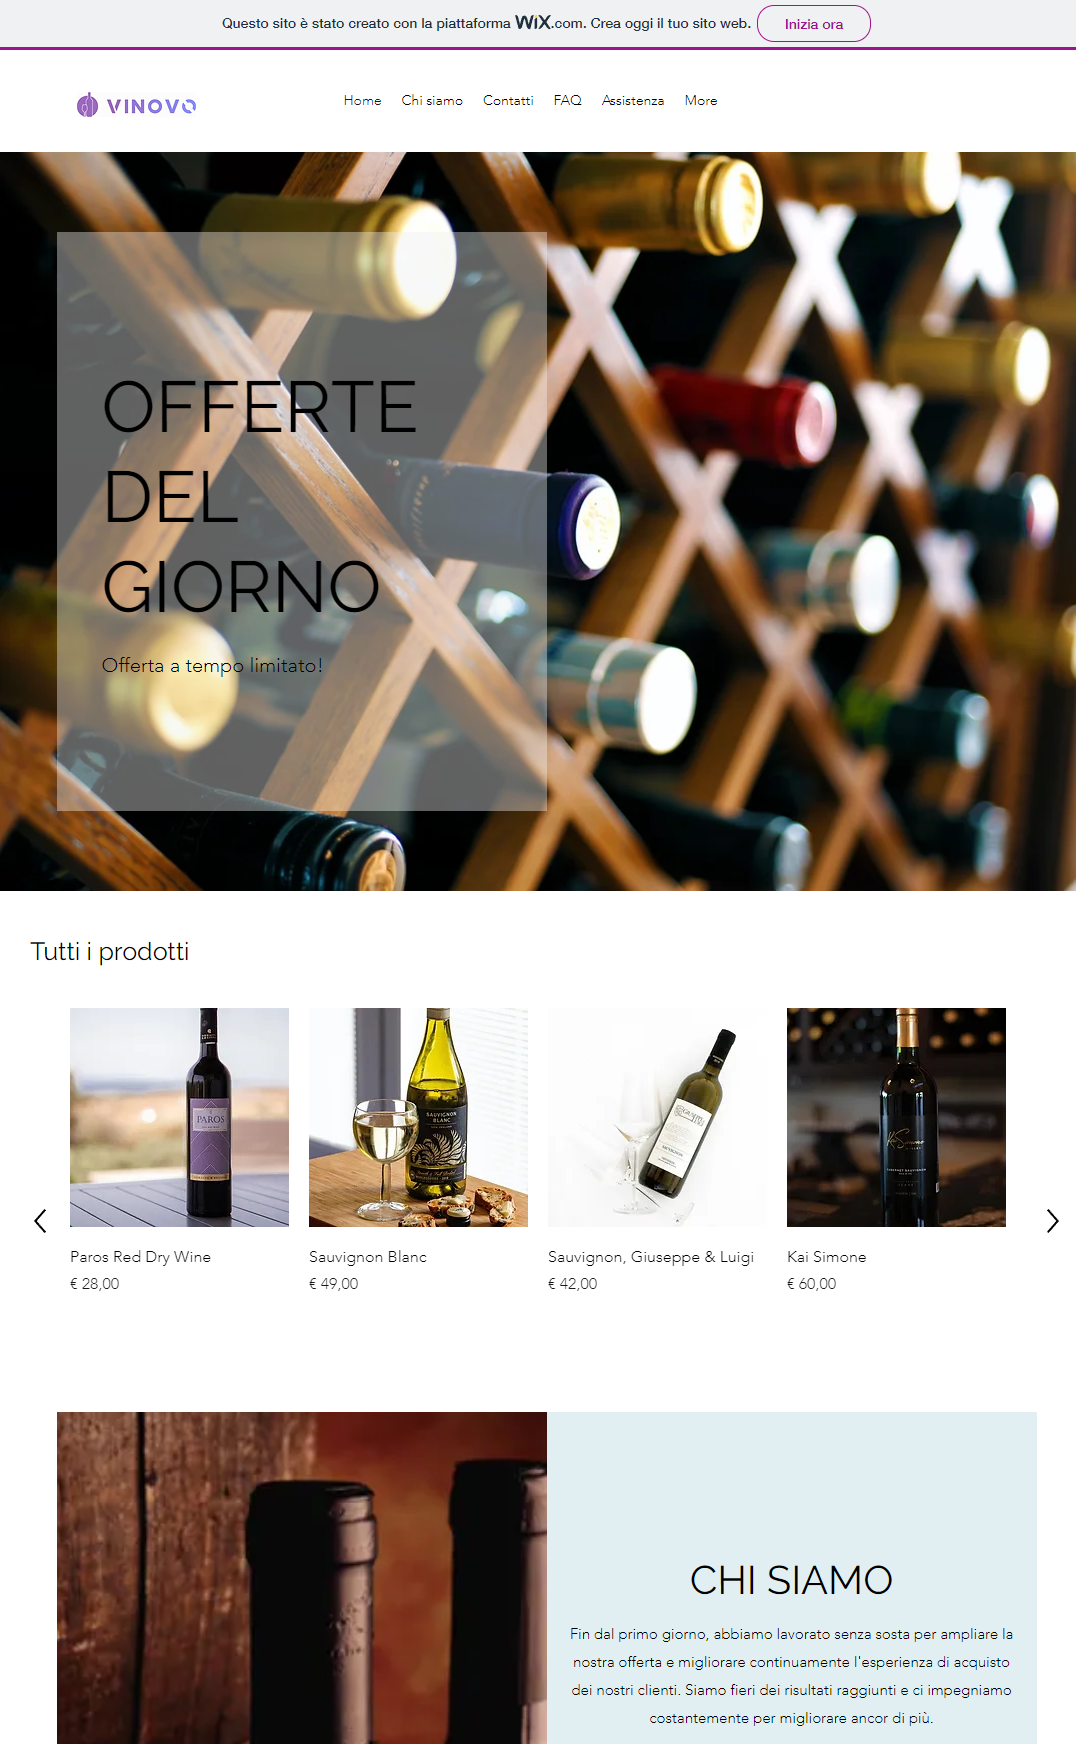
\includegraphics[width=.93\textwidth]{images/sito.png}}
\end{center}


\section{Analisi di mercato}

Il settore vinicolo italiano è un pilastro dell'economia, generando un notevole fatturato annuo di 14,5 miliardi di euro. Da solo, l'export di vino vale 7,1 miliardi di euro, registrando una significativa crescita del 12,4\% nel 2021. Inoltre, la bilancia commerciale dimostra un saldo positivo di circa 6,7 miliardi di euro, confermando l'importanza strategica di questo mercato.

\subsection{Dimensione del mercato}
Il consumo di vino in Italia coinvolge un vasto numero di persone, contando circa 30 milioni di consumatori, che rappresentano il 54\% della popolazione adulta del paese. Questa base di consumatori comprende sia bevitori occasionali che regolari, sottolineando l'ampia diffusione del vino italiano.\\
Un dato interessante è che, attualmente, il 66\% dei consumatori di vino sono uomini. Tuttavia, è degno di nota il fatto che il segmento delle donne sia in forte crescita durante questo decennio, con un aumento del 2,3\%. Le donne stanno assumendo un ruolo sempre più rilevante nel mercato del vino italiano, contribuendo alla sua evoluzione e alla sua diversificazione.\\
Per avere una visione completa del consumo di vino nel paese, si può fare riferimento al grafico che illustra la distribuzione del consumo nelle diverse regioni.
\begin{center}
    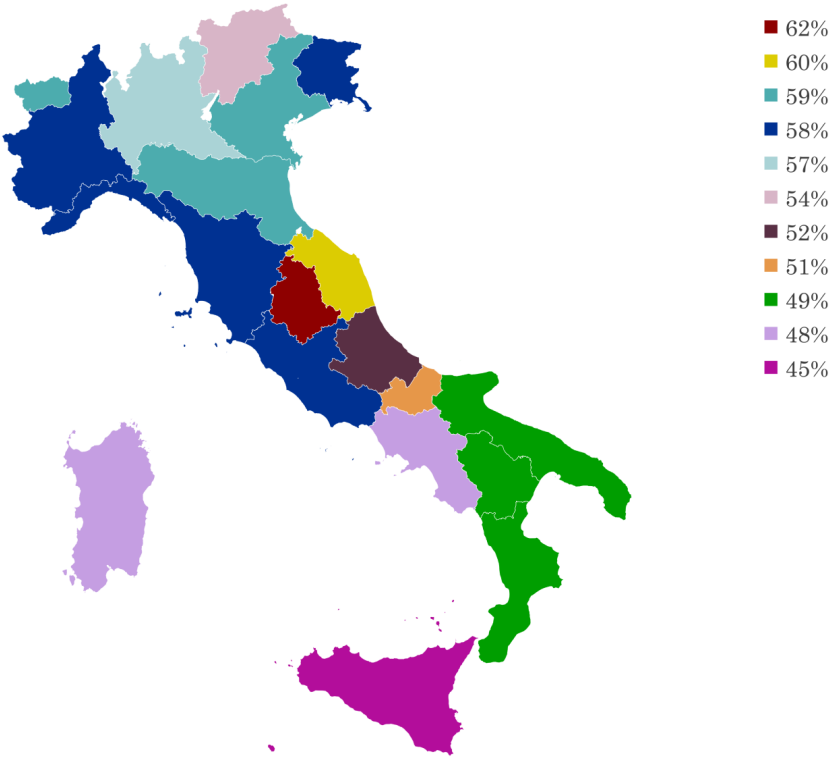
\includegraphics[width=.62\textwidth]{images/grafico_consumatori_regioni.png}
\end{center}
\noindent Dall'analisi del grafico sottostante emerge chiaramente un notevole aumento del consumo di vino da parte dei giovani. Questa tendenza rappresenta un'opportunità significativa per il settore vinicolo, in quanto indica un cambiamento nelle preferenze e nei comportamenti dei consumatori più giovani.\meskip
L'aumento del consumo di vino tra i giovani suggerisce un crescente interesse per la cultura enologica, la scoperta di nuovi sapori e l'esperienza di bevande di alta qualità. Tale tendenza potrebbe essere attribuita a una maggiore consapevolezza dei giovani sui benefici del vino, come le proprietà antiossidanti e la sua associazione con uno stile di vita sofisticato.\meskip
È quindi essenziale adattarsi a questa tendenza, offrendo una selezione di vini adatta ai gusti e alle preferenze dei giovani, utilizzando strategie di marketing mirate e coinvolgenti per catturare l'attenzione di questo segmento di mercato in crescita.\smallskip
\begin{center}
    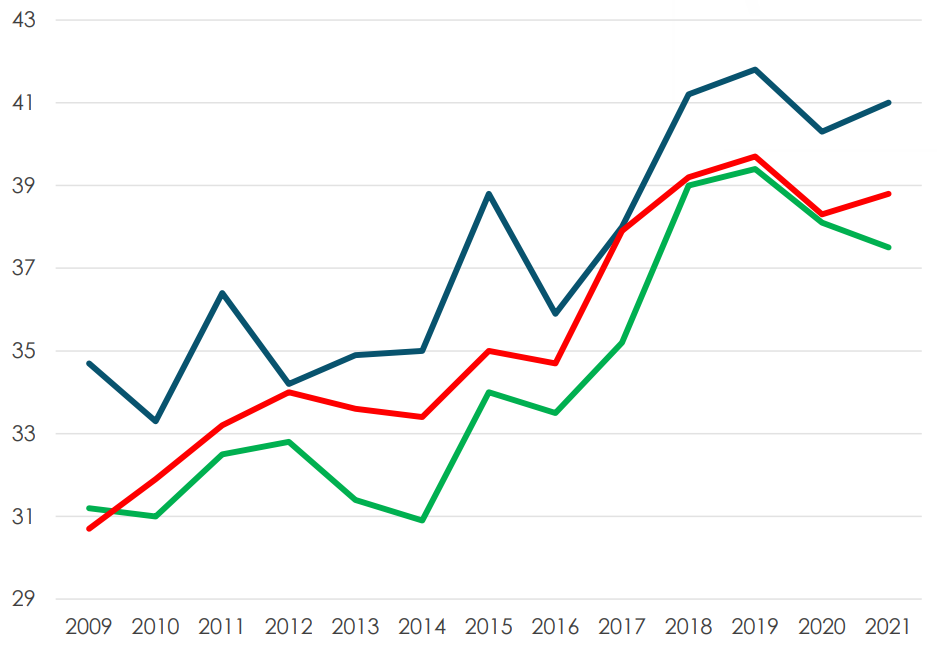
\includegraphics[width=.85\textwidth]{images/consumo_vino_eta.png}
\end{center}
La fascia di consumatori compresa tra i 30 e i 45 anni manifesta un forte interesse per tutti gli aspetti della sostenibilità, inclusi quelli ambientali, economici e sociali. Questi consumatori attribuiscono grande importanza alla provenienza etica dei vini, alle pratiche agricole sostenibili e alla responsabilità sociale delle aziende vinicole. La sostenibilità diventa quindi un fattore decisivo nella scelta dei vini per questa fascia di età.\meskip
D'altra parte, i giovani compresi tra i 18 e i 25 anni mostrano una particolare attrazione verso i vini di prestigio e riconosciuti a livello di brand. Tuttavia, sono anche alla ricerca di nuove esperienze e sono fortemente influenzati dagli eventi e dalle fiere del settore. Questa fascia di consumatori è attiva sui social media, dove seguono influencer del settore vinicolo e cercano informazioni su nuovi vini. È interessante notare che i giovani consumatori, se colpiti positivamente da un vino, tendono a voler approfondire l'esperienza, visitando direttamente le cantine.\meskip
Le donne, in particolare nella fascia di età compresa tra i 30 e i 45 anni, rappresentano oltre il 40\% degli iscritti a degustazioni e corsi di assaggio, ma sono anche la fascia di età che maggiormente apprezza e partecipa a visite aziendali e si avvale dei servizi legati all'Enoturismo.\meskip
Le donne hanno dimostrato una partecipazione attiva nel mondo del vino, sia in termini di formazione sia in termini di esperienze pratiche. Sono sempre più coinvolte in degustazioni guidate, corsi di assaggio e percorsi formativi per approfondire le loro conoscenze sul vino.

\subsection{Analisi PEST}

\subsubsection*{Fattori politici}
Vinovo opera in un'area geografica limitata all'Italia, il che presenta un vantaggio in quanto deve rispettare solo la legislazione nazionale.
La vendita di prodotti online non è soggetta a restrizioni significative, il che semplifica l'ingresso nel mercato, ma allo stesso tempo genera preoccupazione per la facilità con cui nuovi concorrenti potrebbero guadagnare quote di mercato.\\
In Italia, i siti web specializzati nella vendita online devono seguire una specifica normativa fiscale:
\begin{itemize}[itemsep=-5pt, topsep=0pt]
    \item aprire una partita IVA registrandosi presso la Camera di Commercio
    \item le informazioni dell'azienda devono essere chiaramente visibili sul portale online, consentendo agli utenti di trovare facilmente dati come il numero di partita IVA, l'indirizzo della sede legale e il codice di registrazione al Registro delle Imprese.
    \item si deve utilizzare il sistema di fatturazione elettronica, che prevede l'archiviazione digitale delle fatture per un periodo di 10 anni.
\end{itemize}

\subsubsection*{Fattori economici}
È importante tenere in considerazione il cambiamento climatico il quali potrebbe portare a difficoltà e quindi una riduzione significativa della produzione di uva in Italia.\\
Questa riduzione della quantità di uva disponibile potrebbe portare a un aumento dei costi di produzione per le aziende vinicole, in quanto l'offerta di uva è diminuita.\\
Se allo stesso tempo, supponiamo ci sia una crescente domanda di vini italiani all'estero, questo potrebbe portare a un aumento dei prezzi dei vini italiani sul mercato internazionale.
Di conseguenza, le aziende vinicole italiane potrebbero trovarsi ad affrontare costi di produzione più elevati a causa della riduzione dell'offerta di uva e potrebbero anche decidere di aumentare i prezzi dei loro vini per sfruttare la domanda crescente sui mercati internazionali.
Dunque è fondamentale instaurare forti collaborazioni con le aziende vinicole e soprattutto piccoli fornitori.

\subsubsection*{Fattori sociali}
Le preferenze dei consumatori italiani per il vino possono variare in base alle tradizioni regionali, alle abitudini alimentari e alle tendenze di consumo. Vinovo deve adattarsi alle preferenze dei clienti italiani e offrire una gamma di vini che risponda alle diverse esigenze e agli stili di vita dei consumatori locali.\\
Inoltre l'Italia è nota per la sua cultura enogastronomica, e Vinovo può sfruttare l'interesse dei consumatori per i vini italiani di qualità, promuovendo la provenienza, la tradizione e la varietà dei vini offerti.

\subsubsection*{Fattori tecnologici}
In Italia, l'innovazione tecnologica nel settore dell'e-commerce, come miglioramenti nella sicurezza dei pagamenti online, nell'esperienza di acquisto e nella logistica di consegna, influiscono sulla facilità con cui i consumatori possono acquistare vino online.
L'adozione di strumenti digitali e soluzioni tecnologiche nel settore vinicolo può influenzare la competitività della nostra proposta. Ad esempio, l'utilizzo di strumenti di analisi dei dati per comprendere meglio i comportamenti dei clienti e offrire raccomandazioni personalizzate può contribuire al successo di Vinovo.\bigskip
\begin{center}
    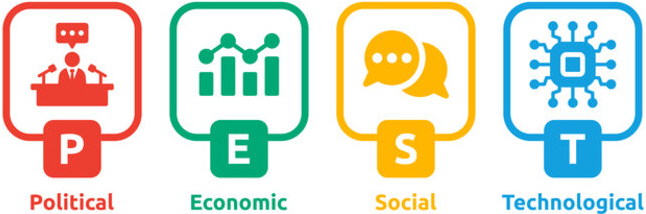
\includegraphics[width=.6\textwidth]{images/pest-analisys.png}
\end{center}

\subsection{Analisi dell'offerta}
In Italia, il mercato del vino è caratterizzato da numerosi produttori privati e piccole enoteche che tradizionalmente vendono i loro prodotti esclusivamente attraverso negozi fisici. Tuttavia, per queste realtà, avviare un proprio e-commerce rappresenta una sfida economica non sostenibile. Di conseguenza, spesso si affidano a piattaforme online già esistenti per raggiungere una clientela più ampia e sfruttare le opportunità offerte dal commercio digitale.

\subsubsection{Analisi dei concorrenti}
Per determinare la quota di mercato che possiamo ottenere, è fondamentale tenere presente che questo segmento di mercato è dominato da aziende consolidate, che vantano un notevole potere di contrattazione sia nei confronti dei clienti che dei fornitori. Nonostante queste sfide, siamo pronti ad affrontare la competizione con innovazione e determinazione. Siamo pronti a sfidare i giganti e a conquistare il nostro spazio nel mercato.\meskip
Sono stati individuati cinque principali concorrenti: Callmewine, Vine.com, Tannico, Xtrawine e Bernabei. Successivamente verranno fornite brevi descrizioni e confronti tra di loro, nonché anche con la nostra startup.\meskip
L'obiettivo è quello di sviluppare una strategia che soddisfi le esigenze dei clienti e offra servizi unici non ancora forniti dai nostri principali concorrenti. Inoltre, l'analisi della concorrenza sarà un processo continuo per rimanere sempre aggiornati e in grado di adattarci al mercato in evoluzione.\meskip
La tabella qui di seguito riassume i principali elementi che distinguono Vinovo dai concorrenti sopra citati:\meskip
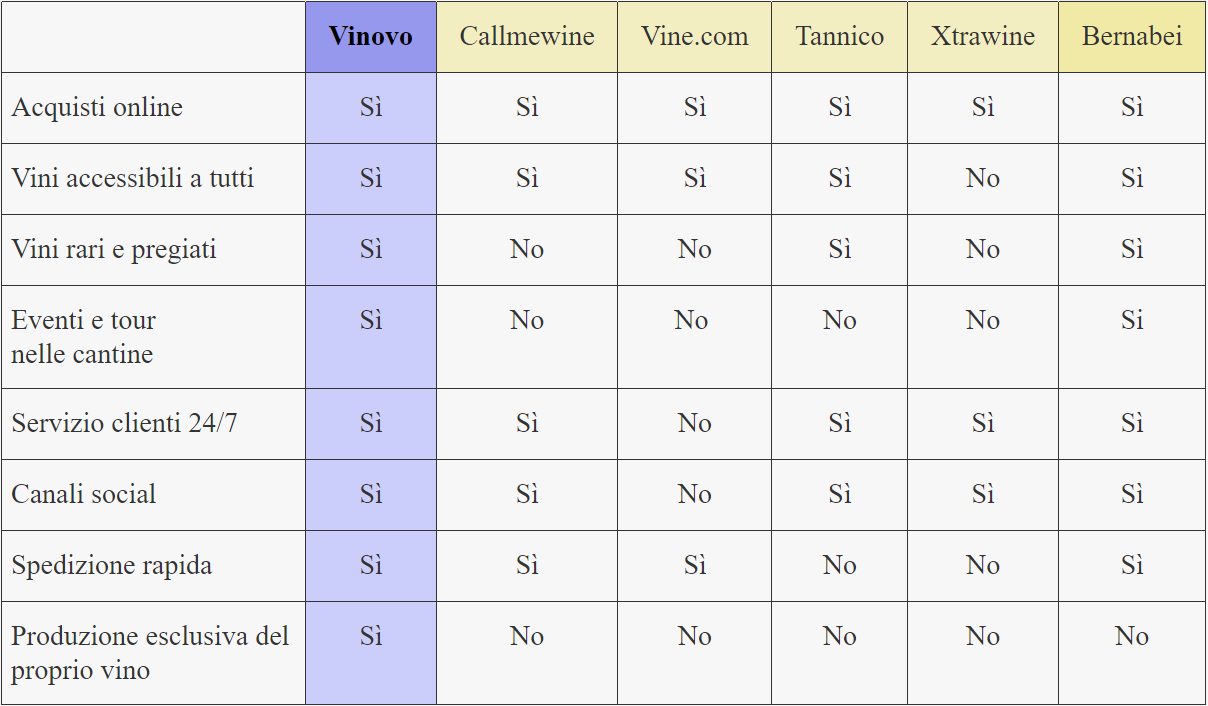
\includegraphics[width=\textwidth]{images/tabella_competitors.png}

\begin{itemize}
    \item \textbf{Callmewine}, è una piattaforma di e-commerce specializzata nella vendita di vini che si colloca tra i leader di mercato in Italia. Possiede un ampio catalogo con circa 11.000 etichette disponibili, che spaziano dai grandi nomi del panorama enologico mondiale ai piccoli produttori, dai distillati di brand più noti a quelli più di nicchia. Possiede quindi una selezione vasta ed eterogenea riuscendo però a guidare l'utente in una scelta consapevole senza disorientarlo, proprio come un vero "sommelier personale".
    \item \textbf{Vino.com} ha lanciato una piattaforma proprietaria multi-brand e multi-channel che ha modernizzato i processi di distribuzione di vino. Oggi \textit{Vino.com} presenta un catalogo di oltre 1.000 cantine e più di 6.000 etichette nazionali e internazionali e il suo fatturato 2020 ha raggiunto i 30 milioni di euro.
    \item \textbf{Tannico} è una delle più ampie enoteche online per offerta di vini italiani nel mondo, con più di 15.000 etichette. Le bottiglie, conservate nel magazzino di Milano, vengono spedite fino a 20 paesi in Europa, e non solo, e provengono da 2.500 cantine attentamente selezionate. Tecnologia, coraggio, innovazione, passione e visione, questi sono i valori con cui l'azienda descrive se stessa e su cui basa il proprio business, con la mission di "raccontare il vino con un linguaggio nuovo".
    \item \textbf{Xtrawine} è un'azienda nata dalla collaborazione di un gruppo di amici sommelier e informatici. Ormai consolidata sul mercato, lo testimoniano le oltre 10.000 referenze e una sede a Hong-kong che proietta le cantine sul mercato cinese; il tutto direttamente dalla piccola città di Forlì.
    \item \textbf{Bernabei} è un enoteca fisica e digitale; conta 5 enoteche fisiche, 5 wine corner e un ottimo e-commerce dove poter comprare oltre al vino, birre, spirits e bibite. Merita particolare attenzione la sezione Caveau con vini rari al suo interno e anche la parte di esperienze: una sezione che ti permette, acquistando il vino di determinate cantine, di poter andare a fare la visita con degustazione gratuitamente in loco.
\end{itemize}
Per concludere l'analisi, è essenziale sottolineare l'importanza dell'attività di differenziazione per mantenere una posizione competitiva nel mercato. Innanzitutto, offrire una spedizione rapida risulta fondamentale non solo per attrarre i clienti più esigenti, ma anche per garantire affidabilità ai ristoranti e locali che collaborano con noi.\meskip
Inoltre, uno dei nostri principali punti di forza è l'esclusività dei nostri vini. Essi vengono prodotti con cura e attenzione dopo un'accurata selezione della materia prima, oltre all'utilizzo di strumentazione all'avanguardia. Questo ci consente di offrire prodotti unici sul mercato, che soddisfano le aspettative dei nostri clienti più esigenti.\meskip
Infine, guardando al futuro, abbiamo l'obiettivo di diversificare le aree geografiche in cui produciamo i nostri vini, al fine di ridurre l'impatto ambientale dei trasporti. Questa strategia ci permetterà di sfruttare le risorse locali e di creare una catena di approvvigionamento più sostenibile, riducendo le distanze di trasporto e promuovendo un'impronta ecologica più ridotta.\bskip
In sintesi, attraverso l'offerta di spedizioni rapide, l'esclusività dei nostri vini e l'attenzione all'impatto ambientale, miriamo a distinguerci nel mercato e a garantire il successo a lungo termine della nostra attività.

\section{Business Model}
In questo capitolo viene presentato il Modello di Business di Vinovo, illustrando la logica fondamentale che ha portato alla creazione del progetto imprenditoriale e la strategia da implementare attraverso strutture organizzative, processi e sistemi, al fine di ottenere un vantaggio competitivo che consenta all'azienda di generare, distribuire e valorizzare i propri prodotti o servizi.

\subsection{Business Model Canvas}
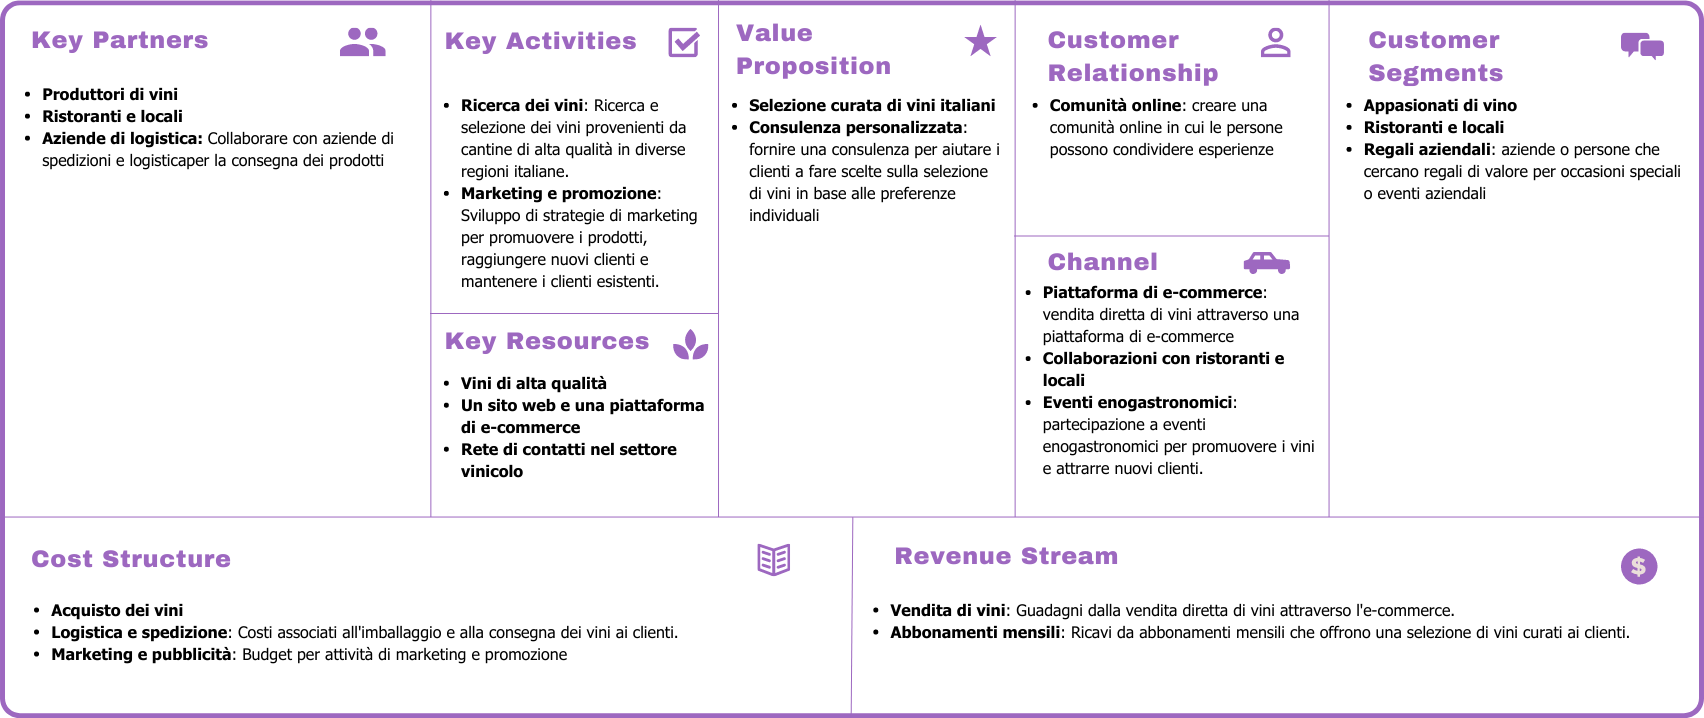
\includegraphics[width=\textwidth]{images/business_model_canvas.png}

\subsubsection{Key Partners}


\subsubsection{Key Activities}


\subsubsection{Key Resources}


\subsubsection{Value Proposition}


\subsubsection{Customer Relationship}


\subsubsection{Channel}


\subsubsection{Customer Segments}


\subsubsection{Cost Structure}


\subsubsection{Revenue Streams}




\end{document}



Per stabilire la quota di mercato che è possibile attaccare è importante considerare che Vinovo è una startup che vuole entrare in un segmento di mercato dominato anche da aziende forti sia dal punto di vista del potere contrattuale verso clienti e fornitori sia dal punto di vista della capacità finanziaria.